\section{Problem 5}

\subsection{Instruction}

The null-to-null bandwidth $B_1$ of the main lobe of the power spectrum
$S_X(f) = T_c sinc^2 (f T_c)$ of a binary random process with chip interval
$T_c$ is $2/T_c$. So, for example, the GPS L1 C/A code, for which
$T_c \approx 1 us$, has $B_1 \approx 2 MHz$. Because of the rounded shape of the
$sinc^2 (f)$ function, the spectrum within $B_1$ is not filled uniformly with
power—in fact, there is very little power at the edges of the $B_1$ interval
where, as it turns out, power matters most for accurate code phase
(i.e., pseudorange) measurements.

Let’s consider a hypothetical radionavigation system with a spreading waveform
that makes more efficient use of the spectrum within $B_1$. Let the (equivalent
baseband) power spectrum of the hypothetical system’s spreading waveform be given
by

\begin{equation}
	S_X(f) = \frac{1}{W} \Pi (f/W)
\end{equation}

This waveform has a two-sided bandwidth of W Hz.


\subsection{MATLAB code}

\begin{lstlisting}
%% Problem 2
% GPS L1 C/A code has a Tc ~ 1us 
% ==> null-to-null bandwidth of the main lobe of the power spectrum (B1)
% B1 = 2/Tc ~ 2 MHz
%
% Note that the spectrum of Sx within B1 is not filled uniformly with power.
%--------------------------------------------------------------------------
clc; close all; clear all
format short
% Since in class we use a different convention for the fourier transform 
% than the one that MATLAB uses by default. Then, I change it right away
oldVal = sympref('FourierParameters',[1 -(2*sym(pi))]);

Tc = 1e-6; W = 2e6;
syms f f1 tau tau1
Sx = Tc*(sinc(f1*Tc))^2;
Sx_efficient = rectangularPulse(f/W)/W; 

figure()
fplot(Sx,[-2/Tc, 2/Tc], Color='k')
hold on
fplot(Sx_efficient,[-2/Tc, 2/Tc], Color='b')
title('Power spectral density')
xlabel('f')
legend('Sx','Sx_{efficient}')
grid on

% a) Find the autocorrelation function Rx(tau) of the spreading waveform by
% taking the inverse transform of Sx(f)
Rx_efficient = ifourier(Sx_efficient,f,tau);

figure()
fplot(Rx_efficient, [-2*Tc, 2*Tc], Color='b')
title('Autocorrelation of Rx_{efficient}')
xlabel('tau')
grid on

% b) How wide is the main peak in the autocorrelation function Rx (from
% first left to first right zero-crossing)?
right_zero_crossing = vpa(solve(Rx_efficient));
main_peak_width = 2*right_zero_crossing % since the function is symmetric

% c) Compare this width to the width of the peak of the autocorrelation
% function Rx_bar for a random binary sequence with a null-to-null
% bandwidth B1 = W
Rx_bar = triangularPulse(-Tc, Tc, tau1); % from class notes

figure()
fplot(Rx_bar,[-2*Tc, 2*Tc], Color='k')
hold on
fplot(Rx_efficient, [-2*Tc, 2*Tc], Color='b')
title('Autocorrelation') 
xlabel('tau')
legend('Rx','Rx_{efficient}')
grid on

main_peak_width_bar = 2*Tc

% d) The following ratio shows that the width of the main peak of the 
% autocorrelation function of the more efficient waveform (in terms of 
% noise) is more than 3 times wider than the original random binary
% sequence. This means that one would loose precision. 
% 
% My logic is the following, one would want the autocorrelation to be a 
% dirac delta. Then, the achieved precision would be excellent. As far as
% one gets from this ideal situation the worse the precision gets.
ratio = main_peak_width / main_peak_width_bar 

\end{lstlisting}

\subsection{Results}

\begin{figure}[H]
	\centering
	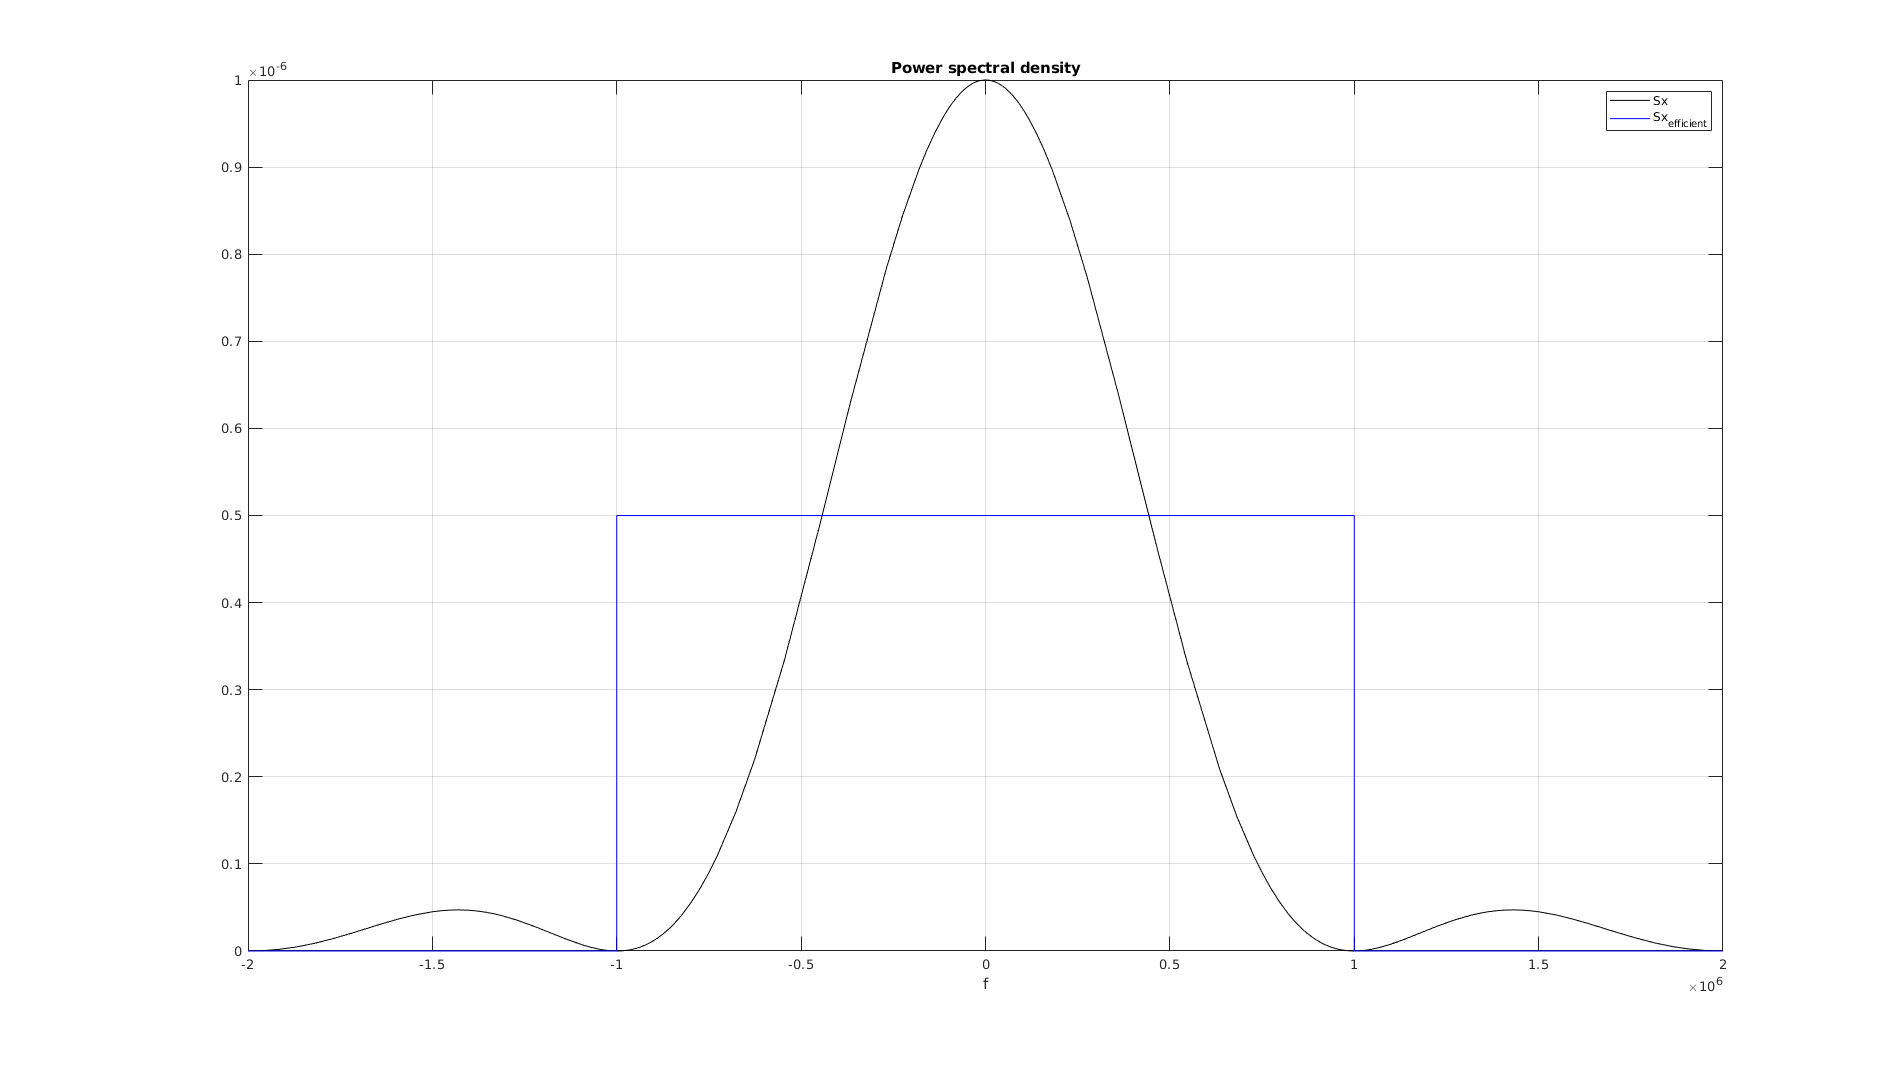
\includegraphics[width=0.9\textwidth]{figs/ex5_psd.png}
	\caption{Power spectral density of X and $X_{eff}$.}
	\label{fig:ex5_psd}
\end{figure}

\subsubsection{Item a, b and c}

(a) Find the autocorrelation function $R_X (\tau )$ of the spreading waveform by
taking the inverse Fourier transform of $S_X (f )$.

(b) How wide is the main peak in the autocorrelation function $R_X (\tau )$
(from first left to first right zero-crossing)?

(c) Compare this width to the width of the peak of the autocorrelation function
$R_X (\tau )$ for a random binary sequence with a null-to-null bandwidth
$B_1 = W$

Figure~\ref{fig:ex5_autocorr} shows the autocorrelation function of the efficient
X and the the one corresponding to a random binary sequence with null-to-null
bandwidth $B_1 = W$.

\begin{figure}[H]
	\centering
	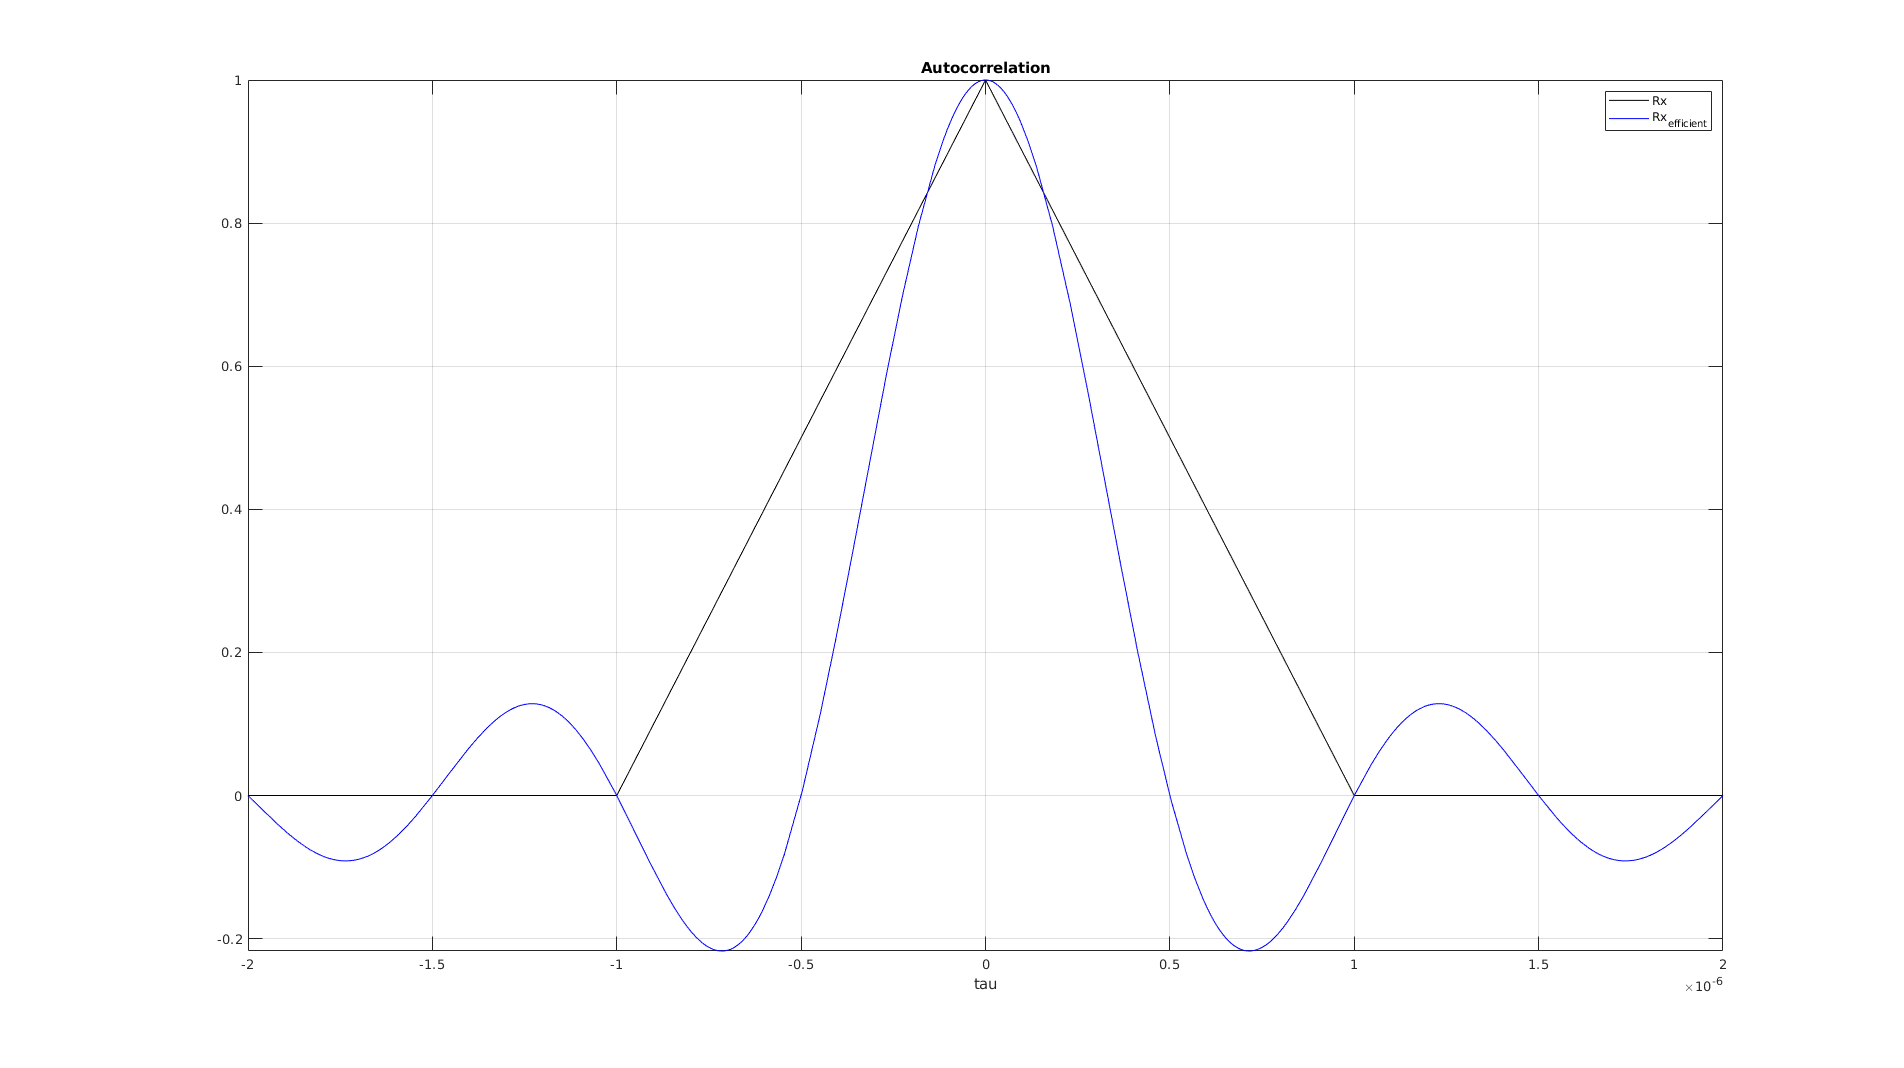
\includegraphics[width=0.9\textwidth]{figs/ex5_autocorr.png}
	\caption{Autocorrelation of X and $X_{eff}$.}
	\label{fig:ex5_autocorr}
\end{figure}

It can be seen from the graph that the main peak in the autocorrelation function
$R_{Xeff} (\tau )$ is equal to $T_c$. On the other hand, the main peak in the
autocorrelation function $R_{X} (\tau )$ is equal to $2*T_c$. Thus, the
width of the main peak of the autocorrelation of $X$ is twice as wide than
$X_{eff}$.

\subsubsection{Item d}

Which of the two autocorrelation functions would lend itself to a more accurate
determination of $\tau peak$, the location of the autocorrelation peak, based on
a single pair of autocorrelation function samples spaced by
$\Delta \tau = 0.2/W seconds$ in a high-C/N0 scenario? Does you answer change for
a low C/N0 scenario? Assume a receiver with a wide front-end bandwidth of 10 W Hz
so that there is not any significant rounding of the triangular autocorrelation
function’s peak. Explain.


The wider your signal is in the time-domain, the narrower it is in the
frequency domain. The narrower the frequency domain, the further away from a
Dirac delta the autocorrelation gets (a Dirac delta is how we would like the
autocorrelation to look like).
However, the wider the signal in the time domain the better would be the
receiver's ability to understand the signal under low C/N0 situations.

Therefore, a tradeoff exists and there's no right answer. I would say
that in a low-C/N0 scenario one should try to slow the sequence down as
much as possible to detect it because detecting it and getting low
accuracy in the range measurement is better than not detecting at all. In
a high-C/N0 I would by greedy with respect to accuracy and make the
spreading code as fast as possible (wide as possible in freq domain).

\subsubsection{Item e}

Why do you suppose the random binary sequence (actually a pseudorandom
approximation of it) was historically used for GPS?

The pseudo-random binary sequence was chosen because of its built-in
ranging capabilities, multiple access characteristic and jamming
rejection. The reason why it needs to be pseudo-random is because without
knowing the actual sequence there's no way to actually "lock" to the
spreading code (no way to have a local replica).

